\begin{frame}
\frametitle{Microreactors}
\begin{columns}
	\column[t]{5cm}
	\begin{itemize}
		\item Several designs are under development in the US.
		\item Plug-and-play reactors.
		\item Remote commercial applications.
		\item Remote military bases.
	\end{itemize}
	\vspace{1cm}
	Features:
	\begin{itemize}
		\item Factory fabricated.
		\item Transportable.
		\item Self-regulating.
	\end{itemize}

    \column[t]{5cm}
	\begin{figure}[htbp!]
		\begin{center}
			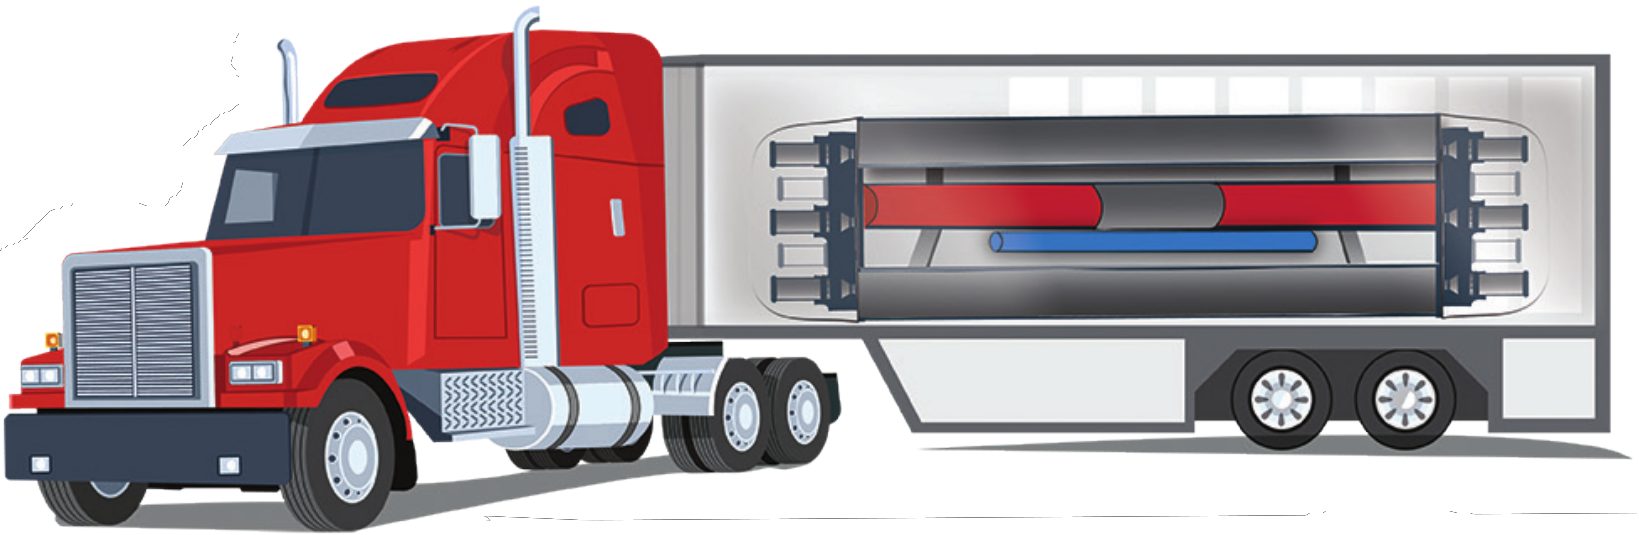
\includegraphics[width=5.2cm]{images/microreactor}
		\end{center}
		\caption{Microreactor design.}
	\end{figure}
\end{columns}
\end{frame}

% should i give a description of different designs??
